\subsection{Glyph: \glyph{Compartment}}\label{sec:compartment}

In order to describe biochemical and cellular events, it is useful to define the notion of pools. A pool is an ensemble of participants that  can be considered to be identical for the events in which they are involved. A compartment is a logical or physical structure that contains pools. A pool can only belong to one compartment. Therefore, the ``same'' biochemical species located in two different compartments are in fact two different pools.

\begin{glyphDescription}

\glyphSboTerm  SBO:0000289 ! functional compartment

\glyphContainer A compartment is represented by a surface enclosed in a continuous border or located between continuous borders. These borders should be noticeably thicker than the borders of the AFNs. A compartment can take \textbf{any} geometry. A compartment must always be entirely enclosed.

\glyphLabel The identification of the compartment is carried by an unbordered box containing a string of characters. The characters can be distributed on several lines to improve readability, although this is not mandatory. The label box can be attached anywhere in the container box. Note that the label can spill-over from the container box.

\glyphAux A \glyph{compartment} can carry a certain number of \glyph{units of information}, that will add information for instance about the physical environment, such as pH, temperature or voltage, see \sect{af:unitInfo}.  The center of the bounding box of a \glyph{unit of information} is located on the mid-line of the border of the compartment.

\end{glyphDescription}

\begin{figure}[H]
  \centering
  \includegraphics[scale = 0.3]{images/compartment}
  \caption{The \AF glyph for \glyph{compartment}.}
  \label{fig:af:compartment}
\end{figure}

